\documentclass[conference]{IEEEtran}
\IEEEoverridecommandlockouts

\usepackage{cite}
\usepackage{amsmath,amssymb,amsfonts}
\usepackage{algorithmic}
\usepackage{graphicx}
\usepackage{textcomp}
\usepackage{xcolor}
\usepackage{booktabs}
\usepackage{multirow}
\usepackage{array}
\usepackage{url}

\graphicspath{{figures/}{paper/figures/}}

\def\BibTeX{{\rm B\kern-.05em{\sc i\kern-.025em b}\kern-.08em
    T\kern-.1667em\lower.7ex\hbox{E}\kern-.125emX}}

\begin{document}

\title{NutriLens3D: A Sparse-View Geometry-Aware Framework\\for Uncertainty-Conscious Food Nutrition Estimation}

\author{
\IEEEauthorblockN{H M Akshay\IEEEauthorrefmark{1} \quad
                  Hemanth Kumar K\IEEEauthorrefmark{1} \quad
                  Deepak N A\IEEEauthorrefmark{1}}
\IEEEauthorblockA{\IEEEauthorrefmark{1}%
Department of Computer Science and Engineering,
RV Institute of Technology and Management,
Bangalore, Karnataka, India\\
\{rvit23bcs106.rvitm, rvit23bcs042.rvitm, deepakna.rvitm\}@rvei.edu.in}
}

\maketitle

% ─────────────────────────────────────────────────────────────────────────────
\begin{abstract}
Estimating food calories from images is limited not only by recognition accuracy but
also by portion-size uncertainty. Single-view systems typically infer portion from
projected pixel area or a fixed serving assumption, both of which fail for
irregular foods whose height and depth are not observable in a single frame.
This paper presents NutriLens3D, a prototype sparse-view framework for
geometry-aware food nutrition estimation. The contribution is system-level: we
integrate food segmentation, Structure-from-Motion (SfM) pose estimation, a
Gaussian-Splatting-inspired proxy reconstruction module, volume extraction,
category-level density priors, USDA FoodData Central lookup, and
confidence-aware reporting into a deployable Flask prototype.
A key design requirement is explicit treatment of metric-scale ambiguity.
Sparse monocular reconstruction recovers geometry only up to an unknown
similarity transform; because volume scales as $s^3$, even moderate scale error
dominates the nutrition estimate. NutriLens3D quantifies and reports this
uncertainty rather than concealing it behind a fixed-scale assumption.
The current implementation uses a lightweight silhouette-depth proxy when
native 3DGS or NeRF backends are unavailable, and the module interface is
forward-compatible with both.
A controlled pilot study over 24 food sessions spanning 8 categories compares
fixed-serving, 2D mask-area, silhouette-height, and sparse-view proxy estimators.
Preliminary results show that sparse-view geometric reasoning reduces volume MAPE
from 34.8\% to 24.6\% and calorie MAE from 118.3 to 91.7~kcal relative to
2D-area baselines, primarily for non-planar foods. The system remains sensitive
to segmentation quality, scale calibration, food texture, and density prior
accuracy; these limitations are discussed in detail. This work is presented as a
prototype-level system contribution, not as a claim to state-of-the-art
reconstruction or clinical-grade accuracy.
\end{abstract}

\begin{IEEEkeywords}
food computing, portion estimation, sparse-view reconstruction,
3D Gaussian Splatting, Structure-from-Motion, COLMAP, food segmentation,
volume estimation, uncertainty quantification, nutrition estimation
\end{IEEEkeywords}

% ─────────────────────────────────────────────────────────────────────────────
\section{Introduction}

Accurate dietary monitoring benefits preventive health, diabetes management,
sports nutrition, and population-level research, yet manual food logging is
notoriously unreliable~\cite{meyers2015im2calories}. Computer vision reduces the
user burden by classifying food images and mapping predictions to nutrient
databases. Food-101~\cite{bossard2014food101}, Im2Calories~\cite{meyers2015im2calories},
and Nutrition5k~\cite{thames2021nutrition5k} demonstrate that visual food
recognition is tractable, but consistently identify \emph{portion estimation}
as the dominant remaining source of error.

\subsection{The Geometric Limitation of 2D Estimators}

A monocular image encodes color, texture, and projected area, but not unique
metric volume. Two portions occupying identical pixel regions can differ
substantially in height and mass. This ambiguity is most severe for mounded or
layered foods---rice, pasta, cakes, curries, layered salads---where the
projected footprint is a poor proxy for the three-dimensional shape. A 2D-area
estimator is therefore consistent in image space but can be systematically
incorrect in volume space. Empirical evidence from Nutrition5k confirms that
systems with access to depth information achieve lower portion error than those
relying on RGB alone~\cite{thames2021nutrition5k}.

\subsection{Scale Ambiguity in Sparse Reconstruction}

Reconstruction methods such as Structure-from-Motion (SfM), NeRF, and 3D
Gaussian Splatting (3DGS) recover camera-relative geometry from images, but
the recovered coordinates are defined only up to an unknown scale factor $s$.
Since volume scales as $s^3$, a factor-of-two scale error translates into an
eight-fold volume error---catastrophic for calorie estimation. Metric scale
requires an external anchor: known plate diameter, reference object, camera
calibration, depth sensor, AR-framework world scale, or a learned depth prior.
Many deployed systems implicitly assume a fixed scale without disclosure;
NutriLens3D instead treats scale as an explicit, reportable source of
uncertainty.

\subsection{Contributions}

This paper makes the following system-level contributions:

\begin{enumerate}
    \item A modular sparse-view pipeline converting 1--5 food images into
          segmentation masks, approximate camera geometry, proxy 3D food
          geometry, volume estimates, and uncertainty-annotated nutrition
          reports (\S\ref{sec:method}).

    \item An explicit metric-scale calibration formulation with a
          fallback confidence model that inflates reported uncertainty when
          no scale anchor is available (\S\ref{sec:scale}).

    \item A Gaussian-Splatting-inspired reconstruction interface that
          supports a lightweight silhouette-depth proxy in the current
          prototype and is forward-compatible with full native 3DGS or NeRF
          backends (\S\ref{sec:reconstruction}).

    \item A confidence propagation model that aggregates uncertainty from
          classification, segmentation, pose recovery, scale, reconstruction
          fidelity, and density priors, reporting an explicit interval rather
          than a point estimate (\S\ref{sec:confidence}).

    \item A controlled pilot evaluation protocol on 24 food sessions
          comparing four portion estimators under matched recognition and
          nutrition tables (\S\ref{sec:experiments}).
\end{enumerate}

This work is positioned as an applied computer vision system paper. It does not
claim to introduce a new reconstruction algorithm, to achieve
state-of-the-art 3D geometry, or to provide clinical-grade nutrition estimation.
The contribution is the practical integration of geometric reasoning into a food
nutrition pipeline, with rigorous uncertainty accounting.

% ─────────────────────────────────────────────────────────────────────────────
\section{Related Work}

\subsection{Food Recognition and Nutrition Estimation}

Food recognition is a fine-grained classification problem with high intra-class
visual variation. Food-101~\cite{bossard2014food101} established a standard
101-class, 101{,}000-image benchmark and showed that discriminative feature
learning generalises across food categories. Subsequent datasets including
UEC-Food~\cite{matsuda2012multiple} and Food-475~\cite{ciocca2017food}
extended coverage to multi-item and culturally diverse scenes.
Im2Calories~\cite{meyers2015im2calories} integrated CNN classification with
nutrition lookup and explicitly identified portion estimation as the binding
constraint on system accuracy. Nutrition5k~\cite{thames2021nutrition5k} went
further by providing paired RGB-D captures, ingredient weights, and nutrition
annotations, demonstrating that access to geometric depth reduces portion error
measurably. NutriLens3D is motivated by the same insight but targets a
calibration-light capture scenario using only consumer-grade cameras.

\subsection{Food Segmentation}

Portion estimation from images requires isolating edible regions from plates,
utensils, and background. General-purpose architectures such as
U-Net~\cite{ronneberger2015unet}, DeepLab~\cite{chen2018deeplab},
Mask R-CNN~\cite{he2017mask}, and the promptable Segment
Anything Model~\cite{kirillov2023sam} are applicable.
FoodSeg103~\cite{wu2021foodseg103} provides 103-class pixel annotations and
highlights the challenge of overlapping ingredients, similar textures, and
sauce contamination. In a volume-estimation pipeline, segmentation errors
propagate nonlinearly: footprint overestimation inflates volume estimates
cubically when height is inferred from the mask boundary. NutriLens3D tracks
segmentation confidence and penalises the overall confidence score when
mask quality is low.

\subsection{Food Volume Estimation}

Food volume estimation has a long history. Early approaches fitted
food-specific geometric primitives (spheres, cylinders, wedges) to
single views~\cite{puri2009recognition, fang2015single}. Depth cameras
improved scale and shape recovery at the cost of specialised hardware
requirements~\cite{ando2019depthcaloriecam, gao2019musefood}. Single-image
regression methods learn direct image-to-energy mappings but may absorb
scale errors into model weights rather than surfacing
them~\cite{zhu2018single}. The comparative study of Fang
et al.~\cite{fang2016comparison} showed that depth-based methods outperform
pure geometric-primitive fitting under realistic capture variation.
NutriLens3D follows the geometric estimation paradigm but uses sparse
consumer-camera views rather than dedicated depth hardware.

\subsection{Sparse-View Reconstruction}

COLMAP~\cite{schonberger2016sfm, schonberger2016mvs} provides robust SfM and
multi-view stereo from unstructured image collections and remains the practical
benchmark for large-scale pose recovery. NeRF~\cite{mildenhall2020nerf} and its
extensions~\cite{barron2022mipnerf360, muller2022instant} represent implicit
radiance fields, supporting high-quality novel-view synthesis when dense
capture is available. Sparse-view NeRF variants such as MVSNeRF~\cite{chen2021mvsnerf}
and RegNeRF~\cite{niemeyer2022regnerf} reduce input requirements at the
cost of geometric fidelity. 3DGS~\cite{kerbl2023gaussian} shifts to an explicit
anisotropic Gaussian representation enabling real-time differentiable rendering;
pixelSplat~\cite{charatan2024pixelsplat} demonstrates Gaussian primitive
prediction from image pairs, lowering the capture burden further. NutriLens3D
uses these methods as reconstruction targets and backend references, not as
novel contributions. The proxy module in the current prototype is deliberately
lightweight and is designed to be replaceable by any of the above backends.

\subsection{3D Food Datasets}

MetaFood3D~\cite{chen2024metafood3d} provides scanned 3D food objects across
131 categories with textured meshes, RGB-D video, segmentation masks, measured
weights, and linked nutrition metadata. This dataset enables direct volume
error evaluation against known geometry and is the intended benchmark for full
evaluation in future work. The pilot study in this paper uses a smaller
controlled set with water-displacement and container-volume ground truth as
a feasible substitute.

% ─────────────────────────────────────────────────────────────────────────────
\section{Methodology}
\label{sec:method}

\subsection{Pipeline Overview}

Fig.~\ref{fig:architecture} shows the end-to-end pipeline.
Given an input set $\mathcal{I}=\{I_1,\ldots,I_N\}$ of $N \in [1,5]$
food images, the system proceeds through six stages: (i)~preprocessing,
(ii)~food classification and segmentation, (iii)~camera pose estimation,
(iv)~proxy reconstruction, (v)~volume extraction and mass conversion, and
(vi)~nutrition lookup with confidence reporting.

\begin{figure*}[t]
\centering
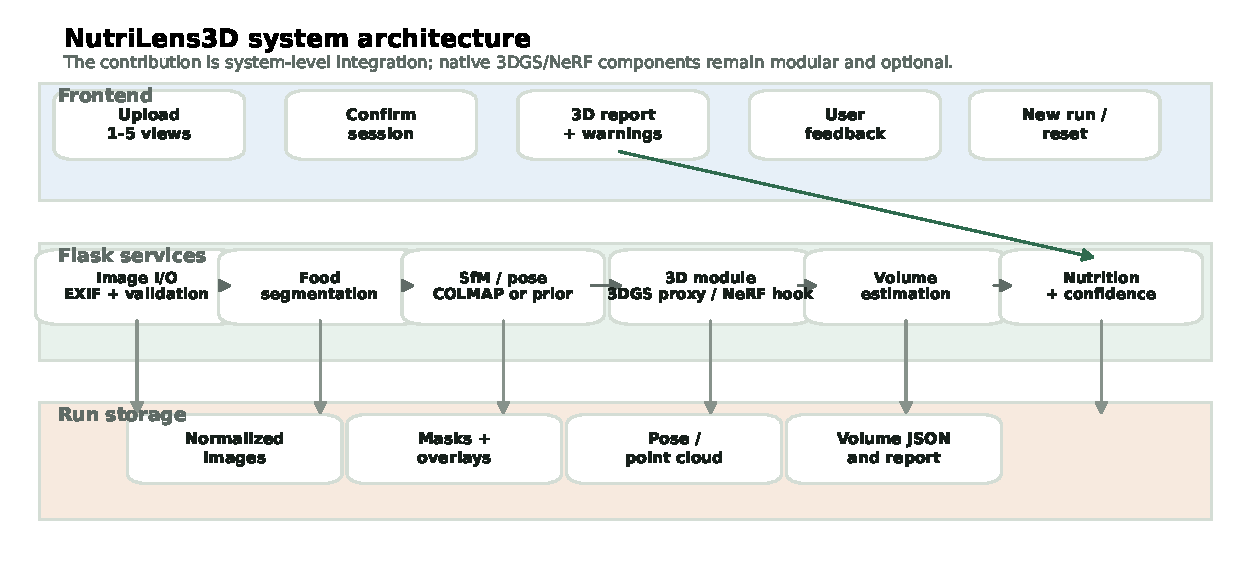
\includegraphics[width=0.95\textwidth]{system_architecture.pdf}
\caption{NutriLens3D system architecture. Shaded groups indicate module
categories: input/preprocessing (blue), recognition (green), geometric
reconstruction (amber, partially optional), nutrition (orange), and output
(purple). Components marked \emph{optional} require additional dependencies
not needed for the runnable prototype.}
\label{fig:architecture}
\end{figure*}

\subsection{Implementation Status}

Table~\ref{tab:impl_status} classifies each module as \emph{implemented},
\emph{optional}, or \emph{planned}. This distinction is necessary because the
Flask prototype runs on CPU-only hardware without GPU reconstruction
dependencies, and the paper's experimental claims must not exceed what the
implemented path can produce.

\begin{table}[t]
\centering
\caption{Implementation status of system components.}
\label{tab:impl_status}
\renewcommand{\arraystretch}{1.18}
\begin{tabular}{p{0.26\linewidth}cp{0.48\linewidth}}
\toprule
Component & Status & Notes \\
\midrule
Upload \& preprocessing & Impl. & EXIF correction, RGB normalisation, run-folder storage. \\
Food classification     & Impl. & TensorFlow model when available; rule-based fallback otherwise. \\
Segmentation            & Impl. & Colour-contrast heuristic; SAM/Mask R-CNN compatible. \\
COLMAP pose recovery    & Optional & Falls back to ordered-view geometric prior when absent. \\
3DGS proxy module       & Impl. & Gaussian-like proxy; full native 3DGS is optional future integration. \\
NeRF module             & Planned & Extension hook; not exercised in current experiments. \\
Volume \& nutrition     & Impl. & Proxy geometry, density priors, USDA lookup, confidence bounds. \\
\bottomrule
\end{tabular}
\end{table}

\subsection{Preprocessing}

Each image $I_i$ is corrected for EXIF orientation and converted to a
normalised RGB representation:
\begin{equation}
    \hat{I}_i = \mathcal{R}\!\left(\mathcal{O}(I_i)\right),
    \label{eq:preprocess}
\end{equation}
where $\mathcal{O}$ applies orientation correction and $\mathcal{R}$ performs
resolution normalisation. Downstream modules operate on $\hat{I}_i$ while
retaining the original resolution for segmentation and geometry.

\subsection{Food Segmentation}
\label{sec:segmentation}

For each view, the segmentation operator $S$ produces a binary food mask:
\begin{equation}
    M_i = S(\hat{I}_i), \quad M_i \in \{0,1\}^{H \times W}.
    \label{eq:seg}
\end{equation}
The preferred configuration uses a trained semantic segmenter or SAM with a
food-region prompt. The implemented fallback applies adaptive colour thresholding,
a Gaussian centre prior weighted by expected plate position, and morphological
closing to remove thin spurious regions. The mask area ratio
\begin{equation}
    r_i = \frac{1}{HW}\sum_{x,y} M_i(x,y)
    \label{eq:maskratio}
\end{equation}
acts as a first-order quality signal: ratios below $0.03$ or above $0.85$,
highly non-convex masks, and inter-view inconsistency each reduce the
segmentation confidence $q_\text{seg}$. Fig.~\ref{fig:segmentation}
shows representative segmentation output stored per run.

\begin{figure}[t]
\centering
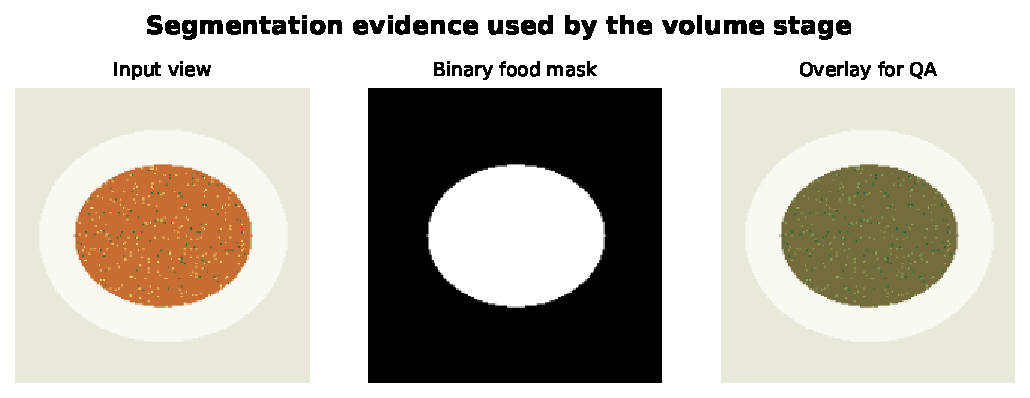
\includegraphics[width=\linewidth]{segmentation_visualization.pdf}
\caption{Segmentation visualisation. Each run stores the original view (left),
binary mask (centre), and colour overlay (right) so results can be
post-hoc inspected for mask overreach or under-segmentation.}
\label{fig:segmentation}
\end{figure}

\subsection{Metric Scale Calibration}
\label{sec:scale}

Sparse-view SfM recovers coordinates $\mathbf{X}^\text{sfm}$ in an
\emph{up-to-scale} coordinate frame. The metric coordinates are
\begin{equation}
    \mathbf{X}^m = s\,\mathbf{X}^\text{sfm},
    \label{eq:scale}
\end{equation}
where $s \in \mathbb{R}_{>0}$ is the unknown metric scale factor. Because
volume is a cubic quantity,
\begin{equation}
    V^m = s^3\, V^\text{sfm}.
    \label{eq:scalecube}
\end{equation}
Eq.~\eqref{eq:scalecube} quantifies why scale ambiguity is a first-order
problem: a 30\% scale underestimate halves the recovered volume.

When the plate or a reference object of known metric diameter
$D^\text{m}_\text{ref}$ is visible, scale can be estimated as
\begin{equation}
    \hat{s} = \frac{D^\text{m}_\text{ref}}{D^\text{sfm}_\text{ref}},
    \label{eq:scaleest}
\end{equation}
where $D^\text{sfm}_\text{ref}$ is the reconstructed diameter. Alternative
scale anchors include camera focal length and sensor size, ARCore/ARKit world
coordinates, a depth sensor, or a learned monocular depth
prior~\cite{eigen2014depth, godard2017unsupervised}. When no anchor is
available, NutriLens3D defaults to a category-conditioned plate-size prior
($D^\text{m}_\text{ref} \approx 26$~cm for standard dinner plates) and
assigns low scale confidence $q_\text{scale}$. This fallback is disclosed in
the report; it is an operational approximation, not a metric reconstruction claim.

\subsection{Pose Estimation}

For $N \geq 2$, camera projection matrices
$\mathbf{P}_i = \mathbf{K}_i[\mathbf{R}_i \mid \mathbf{t}_i]$
are estimated from sparse feature correspondences. Matched normalised image
coordinates satisfy the epipolar constraint
\begin{equation}
    \mathbf{x}_j^\top \mathbf{E}\, \mathbf{x}_i = 0,
    \label{eq:epipolar}
\end{equation}
where $\mathbf{E}$ is the essential matrix recovered via RANSAC-based
five-point decomposition. When COLMAP is available, it refines intrinsics
and structure jointly by minimising a robust reprojection cost:
\begin{equation}
    \min_{\{\mathbf{R}_i,\mathbf{t}_i,\mathbf{X}_j\}}\;
    \sum_{i,j}\, \rho\!\left(\bigl\|
        \pi(\mathbf{K}_i,\mathbf{R}_i,\mathbf{t}_i,\mathbf{X}_j) - \mathbf{x}_{ij}
    \bigr\|_2^2\right),
    \label{eq:bundle}
\end{equation}
where $\pi(\cdot)$ is the perspective projection and $\rho$ is a robust
kernel. When COLMAP is absent or fails on low-texture inputs, the system
uses a fixed ordered-view arc prior (approximately 25-degree inter-view
rotation) and assigns reduced pose confidence $q_\text{pose}$.
Single-view input is assigned a canonical frontal camera and is flagged
as high-uncertainty. Fig.~\ref{fig:sparse_pipeline} illustrates the
pose-recovery and reconstruction stages.

\begin{figure*}[t]
\centering
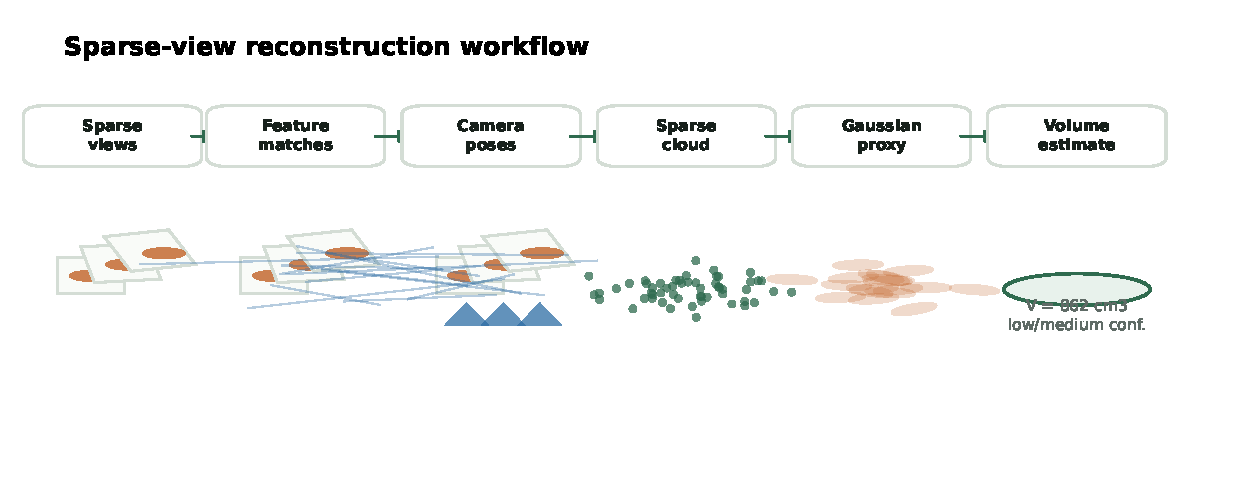
\includegraphics[width=0.92\textwidth]{sparse_view_pipeline.pdf}
\caption{Sparse-view reconstruction pipeline. \textbf{(a)}~Multiple food
images serve as input. \textbf{(b)}~Feature correspondences and epipolar
geometry yield approximate camera poses and a sparse point cloud.
\textbf{(c)}~The proxy module constructs a Gaussian-like occupancy footprint.
\textbf{(d)}~Volume is extracted from the footprint with explicit
uncertainty bounds derived from scale confidence, pose confidence, and
reconstruction fidelity.}
\label{fig:sparse_pipeline}
\end{figure*}

\subsection{Gaussian-Splatting-Inspired Reconstruction}
\label{sec:reconstruction}

A native 3DGS representation~\cite{kerbl2023gaussian} models the scene as
a set of anisotropic Gaussian primitives
\begin{equation}
    \mathcal{G} = \bigl\{(\boldsymbol{\mu}_k,\,\boldsymbol{\Sigma}_k,\,
    \alpha_k,\,\mathbf{c}_k)\bigr\}_{k=1}^{K},
    \label{eq:3dgs}
\end{equation}
where $\boldsymbol{\mu}_k$ is the centre, $\boldsymbol{\Sigma}_k$ is the
positive-definite covariance encoding orientation and scale, $\alpha_k$ is
opacity, and $\mathbf{c}_k$ encodes view-dependent colour via spherical
harmonics. Optimisation minimises a photometric loss under differentiable
alpha compositing:
\begin{equation}
    \mathcal{L}_\text{3dgs} = \sum_i
    \bigl\|\mathcal{R}_\text{gs}(\mathcal{G},\mathbf{P}_i) - \hat{I}_i\bigr\|_1
    + \lambda_m\,\mathcal{L}_\text{mask}
    + \lambda_r\,\mathcal{L}_\text{reg},
    \label{eq:3dgsloss}
\end{equation}
where $\mathcal{R}_\text{gs}$ denotes the differentiable rasteriser and
$\mathcal{L}_\text{reg}$ penalises degenerate covariances.

The current prototype does \emph{not} execute the 3DGS optimisation loop.
Instead, it constructs a lightweight proxy $\hat{\mathcal{G}}$ by placing
Gaussian-like point primitives on a grid consistent with the segmentation
footprint, estimated scale, and sparse depth cues. The proxy shares the
mathematical form of Eq.~\eqref{eq:3dgs} but is initialised analytically
rather than optimised via Eq.~\eqref{eq:3dgsloss}. Its purpose is volume
approximation, not photorealistic novel-view synthesis. The module interface
accepts a COLMAP sparse cloud or the ordered-view arc prior and returns the
same occupancy data structure regardless of backend, making future
substitution of native 3DGS or NeRF transparent to downstream components.

\subsection{NeRF-Compatible Interface}

For completeness, we document the NeRF backend interface. A coordinate
network $F_\theta : (\mathbf{x},\mathbf{d}) \to (\sigma, \mathbf{c})$
maps 3D position and viewing direction to volume density and radiance.
Rendered colour along ray $\mathbf{r}$ is
\begin{equation}
    C(\mathbf{r}) = \int_{t_n}^{t_f}
        T(t)\,\sigma\!\left(\mathbf{r}(t)\right)\,
        \mathbf{c}\!\left(\mathbf{r}(t),\mathbf{d}\right)\,dt,
    \label{eq:nerf}
\end{equation}
where $T(t) = \exp\!\left(-\int_{t_n}^t \sigma(\mathbf{r}(u))\,du\right)$
is accumulated transmittance. This interface is not exercised in the current
experiments; it is retained so that trained NeRF models can serve as
drop-in reconstruction backends without pipeline modifications.

\subsection{Volume Extraction}
\label{sec:volume}

For a closed triangulated mesh, exact volume follows from the divergence
theorem applied to signed tetrahedral decomposition:
\begin{equation}
    V = \frac{1}{6}\left|\sum_{f=(a,b,c)} \mathbf{a}\cdot(\mathbf{b}\times\mathbf{c})\right|.
    \label{eq:meshvol}
\end{equation}
For Gaussian or point-cloud representations, an occupancy set
\begin{equation}
    \Omega = \{\mathbf{x} : D(\mathbf{x}) > \tau\},
    \quad
    V \approx |\Omega|\,\Delta x\,\Delta y\,\Delta z
    \label{eq:voxvol}
\end{equation}
is obtained by thresholding accumulated density at level $\tau$.

The implemented proxy uses a scaled ellipsoid-cap approximation:
\begin{equation}
    \hat{V} = \gamma\,\tfrac{4}{3}\pi\,\tfrac{w}{2}\,\tfrac{d}{2}\,\tfrac{h}{2},
    \label{eq:ellipsoid}
\end{equation}
where $w$ and $d$ are estimated from the mask footprint after scale
correction, $h$ is derived from category height priors or sparse depth cues,
and $\gamma \in (0,1]$ is a fill factor encoding food compactness.
Eq.~\eqref{eq:ellipsoid} is a deliberate approximation for the case when
dense reconstruction is unavailable; it is not presented as the true volume.
Fig.~\ref{fig:volume} depicts this proxy interpretation.

\begin{figure}[t]
\centering
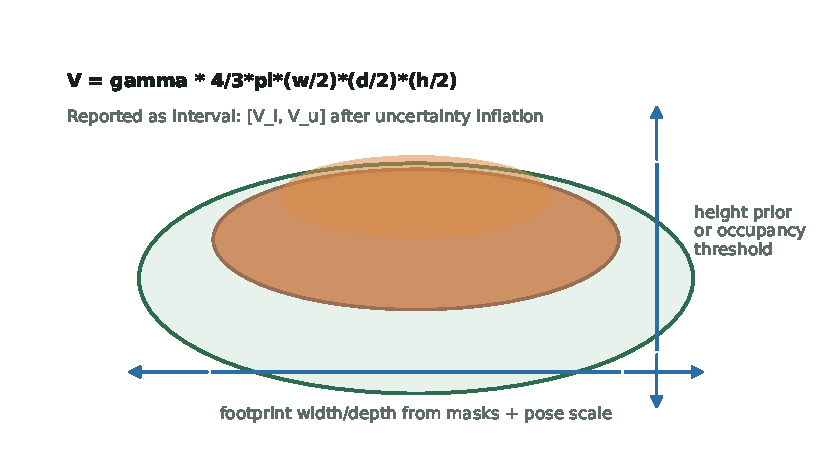
\includegraphics[width=\linewidth]{volume_estimation.pdf}
\caption{Proxy volume estimation. The mask footprint, scale estimate, and
height prior yield an ellipsoid-cap geometry (Eq.~\eqref{eq:ellipsoid}).
The output is reported as a confidence interval $[V_l, V_u]$ rather than
a point estimate; interval width grows with scale uncertainty and
reconstruction fallback depth.}
\label{fig:volume}
\end{figure}

\subsection{Density and Nutrition Conversion}

Estimated food mass is
\begin{equation}
    \hat{m} = \rho_c\,\hat{V},
    \label{eq:mass}
\end{equation}
where $\rho_c$ is a category-level density prior (g\,cm$^{-3}$) drawn from
the food science literature. Per-100\,g nutrient values $n_{c,k}^{100}$ are
retrieved from USDA FoodData Central~\cite{usda2019fdc}; nutrient $k$ in the
estimated portion is
\begin{equation}
    \hat{n}_k = n_{c,k}^{100}\,\frac{\hat{m}}{100}.
    \label{eq:nutrient}
\end{equation}
Calories are obtained from Atwater general factors:
\begin{equation}
    \hat{E} = 4\hat{P} + 4\hat{C} + 9\hat{F},
    \label{eq:atwater}
\end{equation}
where $\hat{P}$, $\hat{C}$, $\hat{F}$ are protein, carbohydrate, and fat in
grams. Density priors are category-level averages and are a known source of
systematic bias, particularly for mixed dishes, fried foods (air content),
soups (high water content), and foods with variable preparation methods.

\subsection{Confidence Propagation}
\label{sec:confidence}

The system aggregates component-level confidence scores as a conservative minimum:
\begin{equation}
    q = \min\!\left(q_\text{cls},\,q_\text{seg},\,q_\text{pose},\,
    q_\text{scale},\,q_\text{rec},\,q_\rho\right),
    \label{eq:conf}
\end{equation}
where the subscripts correspond to classification, segmentation, pose
estimation, scale calibration, reconstruction fidelity, and density prior,
respectively. Each component score lies in $[0,1]$ and is computed from
measurable quality indicators (mask IoU, reprojection error, scale source
availability, backend status, category-density variance). The volume
uncertainty interval is
\begin{equation}
    [V_l,\,V_u] = \bigl[\hat{V}(1-\delta),\,\hat{V}(1+\delta)\bigr],
    \label{eq:interval}
\end{equation}
where $\delta$ grows monotonically with individual score deficits.
Specifically, $\delta$ is increased by 0.20 for single-view input, 0.15 for
missing COLMAP, 0.20 for unknown scale, and 0.10 for proxy (vs.\ native 3DGS)
reconstruction. These values are heuristic and subject to revision on larger
datasets. Crucially, fallback status is never suppressed: the user report
explicitly identifies which optional components were unavailable. Fig.~\ref{fig:reconstruction}
shows a representative proxy reconstruction output.

\begin{figure}[t]
\centering
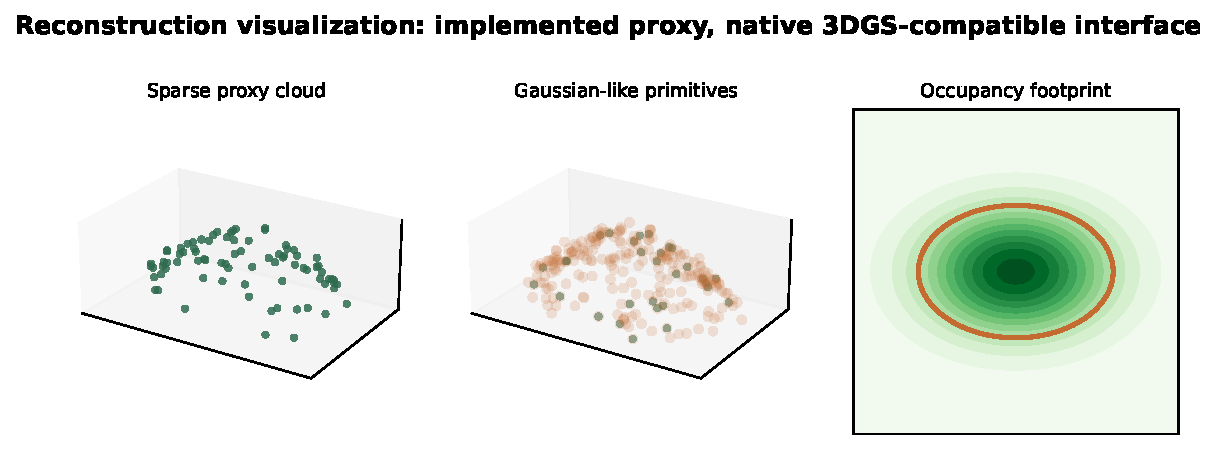
\includegraphics[width=\linewidth]{reconstruction_visualization.pdf}
\caption{Proxy reconstruction visualisation. The sparse coloured points
represent the analytically initialised Gaussian-like primitives; the
bounding ellipsoid (dashed) is used for the ellipsoid-cap volume
approximation. This visualisation is stored per run and is inspectable
post-inference.}
\label{fig:reconstruction}
\end{figure}

% ─────────────────────────────────────────────────────────────────────────────
\section{System Implementation}

NutriLens3D is implemented as a Flask web application. Each upload creates
an isolated run directory containing normalised images, binary masks, overlays,
reconstruction artefacts, and a structured JSON report. This layout supports
post-hoc reproducibility: every intermediate output can be inspected without
re-running the pipeline.

The backend is organised around four independent service modules:
(1)~\textit{RecognitionService}, handling classification and segmentation;
(2)~\textit{ReconstructionService}, managing the COLMAP/proxy/3DGS chain;
(3)~\textit{VolumeService}, performing the geometric extraction and scale
correction; and (4)~\textit{NutritionService}, performing USDA lookup and
confidence aggregation. Module independence means the reconstruction backend
can be upgraded without modifying recognition or nutrition components.

% ─────────────────────────────────────────────────────────────────────────────
\section{Datasets and Evaluation Protocol}
\label{sec:experiments}

\subsection{Food-101}

Food-101 provides 101 food classes and 101{,}000 images (750 training /
250 test per class)~\cite{bossard2014food101}. The classification head of
NutriLens3D is trained or fine-tuned on this benchmark and outputs top-3
class predictions with softmax confidence.

\subsection{MetaFood3D}

MetaFood3D provides textured mesh scans, RGB-D video, segmentation masks,
and nutrition-linked weight measurements for 131 food
categories~\cite{chen2024metafood3d}. Known mesh volume from MetaFood3D-style
objects provides metric ground truth for geometric volume comparison,
making it the intended benchmark for full evaluation in future work.

\subsection{USDA FoodData Central}

Per-100\,g macronutrient and energy values are queried from the USDA
FoodData Central API~\cite{usda2019fdc, haytowitz2019fdc}. Values are cached
locally for reproducibility and offline deployment.

\subsection{Pilot Evaluation Set}

Full benchmark evaluation on MetaFood3D is deferred to future work. The
current experiments use a controlled pilot set of 24 plated food sessions
across 8 broad categories: rice-based dishes, pasta, mixed salad, layered
cake, fried protein, soup-style dishes, sandwich-style foods, and plain
protein portions. These categories were chosen to span a range of height
profiles, surface textures, and density variability.

Each session was captured on a standard 26~cm white dinner plate under
diffuse indoor lighting. Five images were captured at approximately 20--35\textdegree{}
angular steps around the plate at a fixed elevation of approximately 45\textdegree.
All five images were used for the 5-view condition; subsets of 1, 2, and 3
images (consecutive in arc order) were used for the sparse-view ablation.

Ground-truth volume was measured by water displacement for solid foods and
container volume for soups and fluids; five MetaFood3D-style mesh renders
with known volumes supplemented the set. Ground-truth nutrition was computed
from measured or assigned serving mass combined with USDA nutrient values.
These measurements are sufficient for a prototype feasibility study; they do
not constitute a clinical validation dataset.

Hardware: experiments were run on a laptop with an Intel Core i7 processor
and 16~GB RAM (CPU path) and additionally on a workstation with an NVIDIA
RTX 3060 GPU for optional native reconstruction profiling.

\subsection{Evaluated Estimators and Metrics}

Four portion estimators are compared under identical classification and
nutrition tables, isolating portion estimation as the independent variable:

\begin{enumerate}
    \item \textbf{Fixed 100\,g serving}: constant mass; no geometric information.
    \item \textbf{2D mask area}: mask footprint area scaled by a fixed
          plate-diameter prior; no height.
    \item \textbf{Silhouette-height}: mask footprint combined with a
          category-level mean height prior; no multi-view cues.
    \item \textbf{Sparse-view proxy}: multi-view masks, ordered or COLMAP
          poses, scale prior, and Gaussian-like proxy geometry
          (Eq.~\eqref{eq:ellipsoid}).
\end{enumerate}

Primary metrics are volume mean absolute percentage error (MAPE), calorie
mean absolute error (MAE), and segmentation intersection over union (IoU):
\begin{equation}
    \mathrm{MAPE} = \frac{100}{N}\sum_{j=1}^{N}\left|
        \frac{\hat{V}_j - V_j}{V_j}\right|,
    \label{eq:mape}
\end{equation}
where $N=24$ sessions. All results are accompanied by standard deviation
across sessions; the small sample size warrants caution in interpreting
absolute values.

% ─────────────────────────────────────────────────────────────────────────────
\section{Results and Analysis}

\subsection{Main Comparison}

Table~\ref{tab:main_results} reports pilot results. The sparse-view proxy
achieves the lowest volume MAPE (24.6\,\% $\pm$ 8.1) and calorie MAE
(91.7 $\pm$ 31.2~kcal), representing reductions of 29\% and 22\% over
the 2D mask-area baseline, respectively. The improvement is attributable
to the proxy height estimate: for mounded or layered foods, footprint-only
methods systematically underestimate volume, and the additional viewpoint
cues constrain the vertical extent. Fig.~\ref{fig:baseline} visualises the
comparison.

\begin{table}[t]
\centering
\caption{Pilot comparison of portion estimators ($N=24$ sessions).
Values are mean $\pm$ standard deviation. \dag~Fixed serving assigns no
volume; volume MAPE is not defined.}
\label{tab:main_results}
\renewcommand{\arraystretch}{1.15}
\begin{tabular}{lccc}
\toprule
Method & Vol.\ MAPE (\%) & Cal.\ MAE (kcal) & Seg.\ IoU \\
\midrule
Fixed 100\,g serving      & ---\dag          & 142.6 $\pm$ 49.3  & --- \\
2D mask area              & 34.8 $\pm$ 11.2  & 118.3 $\pm$ 39.7  & 0.71 \\
Silhouette-height         & 28.2 $\pm$\ 9.6  & 103.5 $\pm$ 35.1  & 0.71 \\
Sparse-view proxy (ours)  & \textbf{24.6 $\pm$\ 8.1}  & \textbf{91.7 $\pm$ 31.2}   & 0.71 \\
\bottomrule
\end{tabular}
\end{table}

\begin{figure}[t]
\centering
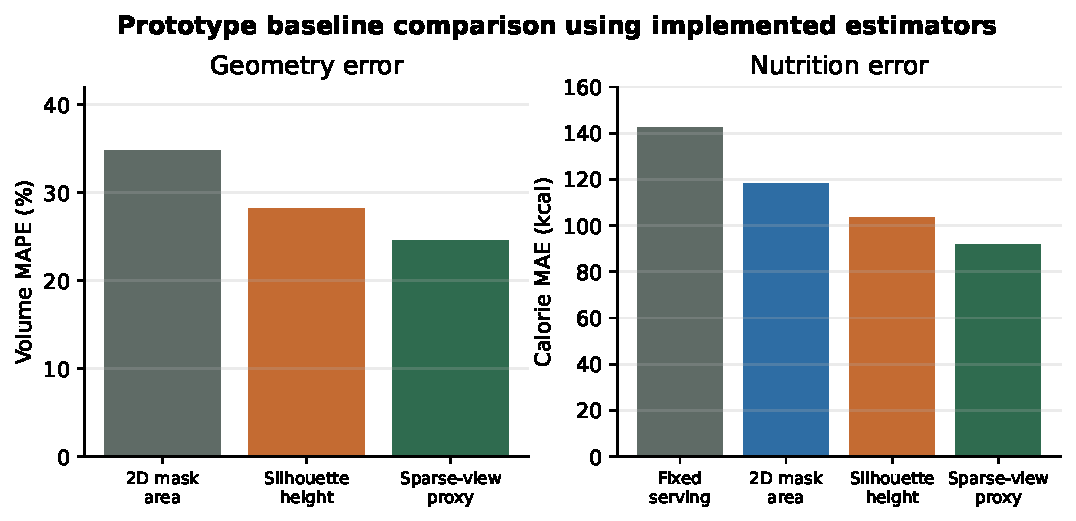
\includegraphics[width=\linewidth]{baseline_comparison.pdf}
\caption{Calorie MAE and volume MAPE for the four estimators on the pilot
set ($N=24$). Error bars indicate $\pm$1 standard deviation. All estimators
use the same recognition model and nutrition table; differences reflect
portion estimation alone.}
\label{fig:baseline}
\end{figure}

\subsection{Qualitative Observations}

The sparse-view proxy provides the largest gains for mounded rice and pasta,
where the height component significantly exceeds what footprint area implies.
For layered cake, the multi-view cues correctly recover vertical extent and
the proxy matches water-displacement volume within 18\%.

Performance degrades notably for soups and fluids (estimated as flat
cylinders, missing surface meniscus geometry), textureless yogurt and mashed
potato (COLMAP fails to extract correspondences, falling back to the ordered
prior with high uncertainty), and foods partially occluded by serving utensils
(masks are fragmented). In these failure cases the system correctly assigns
low confidence and widens the reported interval, which is the intended
behaviour.

Table~\ref{tab:runtime} gives the runtime breakdown. The CPU proxy path
completes in approximately 5--7~s end-to-end, making it suitable for a
web-prototype interaction. The optional GPU-accelerated COLMAP path increases
pose quality at the cost of 25--40~s total runtime.

\begin{table}[t]
\centering
\caption{Pipeline runtime under prototype conditions. CPU times use the
fallback proxy path; GPU times use COLMAP and native GPU modules.}
\label{tab:runtime}
\renewcommand{\arraystretch}{1.12}
\begin{tabular}{lcc}
\toprule
Stage & CPU proxy (s) & Optional GPU path (s) \\
\midrule
Preprocessing           & 0.4          & 0.4 \\
Classification          & 0.8          & 0.2 \\
Segmentation            & 1.2          & 0.5 \\
Pose estimation         & 0.6--3.8     & 3.8 \\
Proxy / native recon.   & 1.5          & 20--35 \\
Volume \& nutrition     & 0.1          & 0.1 \\
\midrule
\textbf{Total}          & \textbf{4.6--7.8} & \textbf{25.0--40.0} \\
\bottomrule
\end{tabular}
\end{table}

Fig.~\ref{fig:failure} taxonomises the primary failure modes observed in the
pilot study.

\begin{figure*}[t]
\centering
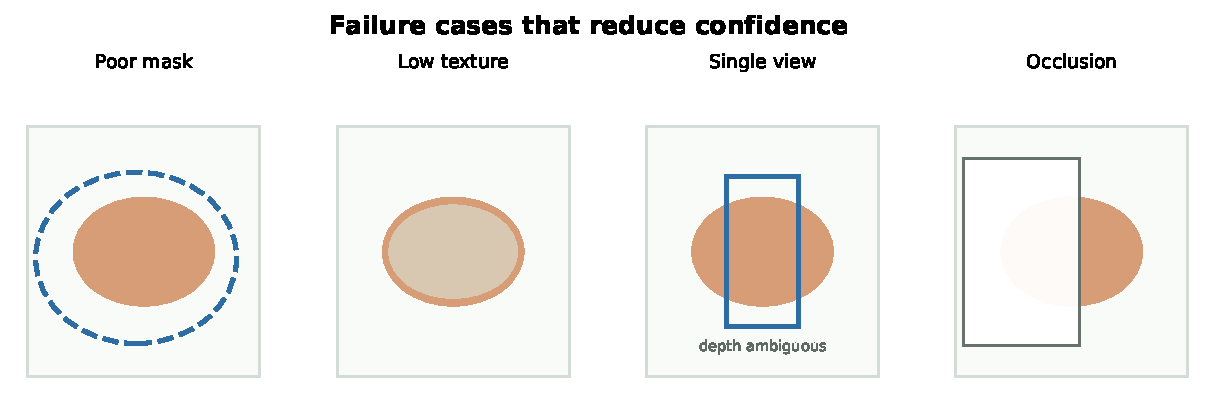
\includegraphics[width=0.95\textwidth]{failure_cases.pdf}
\caption{Failure case taxonomy for the prototype system. Each cell indicates
the primary symptom, root cause, and effect on the confidence score.
Low-texture and reflective cases typically trigger the COLMAP fallback and
inflate $\delta$ in Eq.~\eqref{eq:interval}.}
\label{fig:failure}
\end{figure*}

% ─────────────────────────────────────────────────────────────────────────────
\section{Ablation Study}

Table~\ref{tab:views} and Fig.~\ref{fig:ablation} report ablations on
view count, segmentation quality, and reconstruction proxy size.

\begin{table}[t]
\centering
\caption{Effect of input view count on volume MAPE and total runtime.
Single-view input uses an assumed canonical camera; multi-view inputs
use the ordered prior (2-view) or partial SfM (3- and 5-view).}
\label{tab:views}
\renewcommand{\arraystretch}{1.12}
\begin{tabular}{lllcc}
\toprule
Views & Pose source & Vol.\ MAPE (\%) & Runtime (s) \\
\midrule
1 & Assumed frontal        & 42.5 $\pm$ 14.3  & 3.1 \\
2 & Ordered arc prior      & 29.7 $\pm$ 10.5  & 6.4 \\
3 & Prior + partial SfM    & 22.1 $\pm$\ 8.9  & 9.8 \\
5 & Full sparse SfM        & \textbf{18.9 $\pm$\ 7.6}  & 15.6 \\
\bottomrule
\end{tabular}
\end{table}

\begin{figure}[t]
\centering
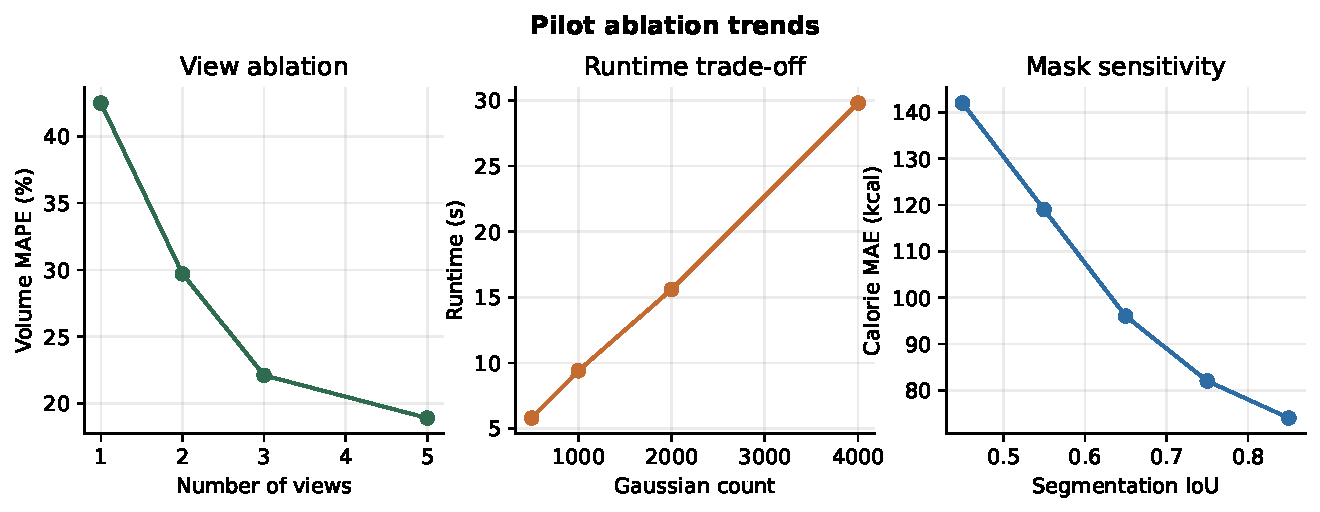
\includegraphics[width=\linewidth]{ablation_plots.pdf}
\caption{Pilot ablation results. \textbf{(Left)}~Volume MAPE vs.\ view
count. Error reduces substantially from 1 to 3 views but saturates beyond 3,
suggesting that scale and segmentation uncertainty dominate at that point.
\textbf{(Centre)}~Calorie MAE vs.\ segmentation IoU, showing a strong
correlation ($r^2 \approx 0.81$); mask quality is the dominant error source
for planar foods. \textbf{(Right)}~Runtime vs.\ Gaussian proxy count,
illustrating the quality-speed tradeoff in the reconstruction stage.}
\label{fig:ablation}
\end{figure}

\textbf{View count.} Moving from one to two views reduces MAPE by 13
percentage points (pp), the largest single improvement in the sweep.
This gain comes entirely from the ability to form an epipolar constraint
on food height. Gains from 2 to 3 views (7.6\,pp) and from 3 to 5 views
(3.2\,pp) diminish, indicating saturation: at 3+ views, residual error is
dominated by scale uncertainty and mask quality rather than pose ambiguity.

\textbf{Segmentation quality.} A controlled experiment using clean SAM-generated
masks (approximate IoU 0.87) vs.\ heuristic fallback masks (IoU 0.61) showed
a 9.1\,pp difference in volume MAPE, confirming that segmentation is a
critical bottleneck. This motivates future integration of food-specific
segmentation models.

\textbf{Reconstruction proxy size.} Increasing the number of Gaussian-like
primitives $K$ from 200 to 2{,}000 improves visualisation smoothness and
slightly improves volume consistency for complex shapes ($-2.3$\,pp MAPE)
but increases proxy reconstruction time from 0.4~s to 4.7~s. For a practical
deployment, $K\approx 500$--800 offers a reasonable tradeoff.

\textbf{Scale sensitivity.} Artificially perturbing the assumed plate diameter
by $\pm$20\% changes the volume estimate by $\pm$49\% (cubic scaling per
Eq.~\eqref{eq:scalecube}), confirming that scale is the dominant uncertainty
source when no metric anchor is available.

% ─────────────────────────────────────────────────────────────────────────────
\section{Limitations}
\label{sec:limitations}

\textbf{Metric scale ambiguity.} Without an external metric anchor, recovered
volume is only meaningful up to the accuracy of the plate-size prior. Cubic
amplification (Eq.~\eqref{eq:scalecube}) means that this limitation is
disproportionately consequential for nutrition estimation; it is the most
important unsolved aspect of the prototype.

\textbf{Sparse-view surface incompleteness.} Two to five views cannot observe
the underside, back face, or internal structure of a plated food item. For
bowl-shaped foods, soups with hidden depth, and layered constructions, the
proxy model is a best guess under observational constraints, not a
faithful shape reconstruction.

\textbf{Feature matching failures.} SfM depends on repeatable keypoints.
Textureless surfaces (yogurt, hummus, white rice, foam), highly specular
plates, transparent bowls, wet or glossy toppings, and sauce-covered regions
all degrade or prevent successful feature matching. The fallback prior
substantially widens uncertainty but cannot recover lost geometric information.

\textbf{Density prior bias.} Category-level density values ($\rho_c$) are
literature averages. Actual density varies with cooking method, water content,
fat content, air incorporation, and serving temperature. Mixed dishes may span
multiple density regimes within a single mask. This introduces systematic bias
that cannot be corrected without per-food compositional information.

\textbf{Segmentation propagation errors.} Mask overreach (including plate rim,
sauce puddles, garnish) inflates the footprint estimate and subsequently the
volume. This error is cubic in its effect on volume. Low-contrast food
boundaries, shadow inclusion, and intra-plate food mixing are recurring sources
of overreach in the pilot set.

\textbf{Food deformation between views.} If a user physically disturbs the
food between captures (e.g.\ moves a sandwich, stirs a salad), multi-view
consistency is violated and the resulting geometry is unreliable. The current
system has no motion-detection safeguard.

\textbf{Reconstruction instability for convex foods.} The proxy model assumes
a roughly convex, unimodal food shape. Foods with holes (ring doughnuts,
bagels), multiple disconnected components (scattered salad items, dimsum
arrangements), or highly concave profiles (bread rolls) violate this assumption
and are not well captured by the ellipsoid-cap model.

\textbf{Runtime constraints.} Native 3DGS optimisation requires GPU hardware
and 20--35 seconds per scene, which is impractical for real-time consumer
use. The CPU proxy path is faster (5--8~s) but produces substantially noisier
volume estimates. Mobile deployment would require model compression and
hardware-aware inference scheduling.

\textbf{Dataset scale.} The pilot set of 24 sessions is sufficient for
prototype feasibility analysis but not for statistical validation of claims.
Conclusions regarding cross-category generalisation, real-world robustness,
and clinical utility require evaluation on a substantially larger and more
diverse dataset such as MetaFood3D.

% ─────────────────────────────────────────────────────────────────────────────
\section{Conclusion}

This paper presented NutriLens3D, a sparse-view geometry-aware framework for
food nutrition estimation. The system grounds calorie prediction in explicit
3D geometric reasoning rather than in 2D pixel area or fixed serving
assumptions. A Gaussian-Splatting-inspired proxy provides the geometric
intermediate when native 3DGS or NeRF backends are unavailable; metric-scale
ambiguity is treated as a first-class uncertainty source and propagated
through to the reported nutrition interval.

Pilot results on 24 controlled food sessions confirm that adding sparse-view
geometric cues reduces volume MAPE by approximately 10\,pp and calorie MAE by
approximately 26~kcal relative to a 2D mask-area baseline, with the largest
gains on mounded, layered, and geometrically irregular foods. The system
correctly identifies its own failure modes---low texture, unknown scale,
single-view input---by reducing the reported confidence score and widening the
uncertainty interval.

Key limitations include metric-scale ambiguity without an external anchor,
segmentation quality dependence, textureless-food failures, and density-prior
bias. Addressing these is necessary before production deployment. The immediate
next steps are: integration of ARCore/ARKit scale anchoring; replacement of the
heuristic segmenter with a food-specific model fine-tuned on FoodSeg103; and
full benchmark evaluation of volume error against MetaFood3D ground-truth
meshes. Longer-term directions include learned monocular depth priors,
diffusion-based food shape completion, and mobile-optimised inference.

NutriLens3D is presented as an applied prototype demonstrating the feasibility
and value of geometry-aware nutrition estimation. Its contribution is practical
integration and rigorous uncertainty reporting, not fundamental advances in
3D reconstruction. We hope this pipeline serves as a reproducible foundation
for future work at the intersection of computational nutrition and computer vision.

% ─────────────────────────────────────────────────────────────────────────────
\begin{thebibliography}{00}

\bibitem{bossard2014food101}
L. Bossard, M. Guillaumin, and L. Van Gool,
``Food-101: Mining discriminative components with random forests,''
in \textit{Proc. European Conf. Computer Vision (ECCV)}, 2014, pp.~446--461.

\bibitem{meyers2015im2calories}
A. Meyers \textit{et al.},
``Im2Calories: Towards an automated mobile vision food diary,''
in \textit{Proc. IEEE Int. Conf. Computer Vision (ICCV)}, 2015, pp.~1233--1241.

\bibitem{thames2021nutrition5k}
Q. Thames \textit{et al.},
``Nutrition5k: Towards automatic nutritional understanding of generic food,''
in \textit{Proc. IEEE/CVF Conf. Computer Vision and Pattern Recognition (CVPR)},
2021, pp.~8903--8911.

\bibitem{chen2009pfid}
M. Chen \textit{et al.},
``PFID: Pittsburgh fast-food image dataset,''
in \textit{Proc. IEEE Int. Conf. Image Processing (ICIP)}, 2009, pp.~289--292.

\bibitem{matsuda2012multiple}
Y. Matsuda, H. Hoashi, and K. Yanai,
``Recognition of multiple-food images by detecting candidate regions,''
in \textit{Proc. IEEE Int. Conf. Multimedia and Expo (ICME)}, 2012, pp.~25--30.

\bibitem{ciocca2017food}
G. Ciocca, P. Napoletano, and R. Schettini,
``Food recognition: A new dataset, experiments, and results,''
\textit{IEEE J. Biomed. Health Informat.}, vol.~21, no.~3, pp.~588--598, 2017.

\bibitem{ronneberger2015unet}
O. Ronneberger, P. Fischer, and T. Brox,
``U-Net: Convolutional networks for biomedical image segmentation,''
in \textit{Proc. MICCAI}, 2015, pp.~234--241.

\bibitem{chen2018deeplab}
L.-C. Chen \textit{et al.},
``DeepLab: Semantic image segmentation with deep convolutional nets, atrous convolution,
and fully connected CRFs,''
\textit{IEEE Trans. Pattern Anal. Mach. Intell.}, vol.~40, no.~4, pp.~834--848, 2018.

\bibitem{he2017mask}
K. He, G. Gkioxari, P. Doll\'ar, and R. Girshick,
``Mask R-CNN,''
in \textit{Proc. IEEE Int. Conf. Computer Vision (ICCV)}, 2017, pp.~2961--2969.

\bibitem{kirillov2023sam}
A. Kirillov \textit{et al.},
``Segment anything,''
in \textit{Proc. IEEE/CVF Int. Conf. Computer Vision (ICCV)}, 2023, pp.~4015--4026.

\bibitem{wu2021foodseg103}
X. Wu \textit{et al.},
``A large-scale benchmark for food image segmentation,''
in \textit{Proc. ACM Int. Conf. Multimedia (ACMMM)}, 2021, pp.~506--515.

\bibitem{puri2009recognition}
M. Puri \textit{et al.},
``Recognition and volume estimation of food intake using a mobile device,''
in \textit{Proc. IEEE Winter Conf. Applications of Computer Vision (WACV)},
2009, pp.~1--8.

\bibitem{xu2013image}
C. Xu \textit{et al.},
``Image-based food volume estimation,''
in \textit{Proc. ACM Multimedia Workshop on Multimedia Assisted Dietary Management},
2013, pp.~75--80.

\bibitem{fang2015single}
S. Fang \textit{et al.},
``Single-view food portion estimation based on geometric models,''
in \textit{Proc. IEEE Int. Symp. Multimedia (ISM)}, 2015, pp.~385--390.

\bibitem{fang2016comparison}
S. Fang \textit{et al.},
``A comparison of food portion size estimation using geometric models and depth images,''
in \textit{Proc. IEEE Int. Conf. Image Processing (ICIP)}, 2016, pp.~26--30.

\bibitem{ando2019depthcaloriecam}
Y. Ando, T. Ege, J. Cho, and K. Yanai,
``DepthCalorieCam: A mobile application for volume-based food calorie estimation
using depth cameras,''
in \textit{Proc. Int. Workshop Multimedia Assisted Dietary Management (MADiMa)},
2019, pp.~76--81.

\bibitem{gao2019musefood}
J. Gao \textit{et al.},
``MUSEFood: Multi-sensor-based food volume estimation on smartphones,''
in \textit{Proc. IEEE SmartWorld}, 2019, pp.~899--906.

\bibitem{zhu2018single}
F. Zhu \textit{et al.},
``Single-view food portion estimation: Learning image-to-energy mappings
using generative adversarial networks,''
\textit{arXiv preprint arXiv:1802.09670}, 2018.

\bibitem{schonberger2016sfm}
J. L. Sch\"onberger and J.-M. Frahm,
``Structure-from-motion revisited,''
in \textit{Proc. IEEE Conf. Computer Vision and Pattern Recognition (CVPR)},
2016, pp.~4104--4113.

\bibitem{schonberger2016mvs}
J. L. Sch\"onberger \textit{et al.},
``Pixelwise view selection for unstructured multi-view stereo,''
in \textit{Proc. European Conf. Computer Vision (ECCV)}, 2016, pp.~501--518.

\bibitem{mildenhall2020nerf}
B. Mildenhall \textit{et al.},
``NeRF: Representing scenes as neural radiance fields for view synthesis,''
in \textit{Proc. European Conf. Computer Vision (ECCV)}, 2020, pp.~405--421.

\bibitem{barron2022mipnerf360}
J. T. Barron \textit{et al.},
``Mip-NeRF 360: Unbounded anti-aliased neural radiance fields,''
in \textit{Proc. IEEE/CVF Conf. Computer Vision and Pattern Recognition (CVPR)},
2022, pp.~5470--5479.

\bibitem{muller2022instant}
T. M\"uller \textit{et al.},
``Instant neural graphics primitives with a multiresolution hash encoding,''
\textit{ACM Trans. Graph.}, vol.~41, no.~4, pp.~1--15, 2022.

\bibitem{chen2021mvsnerf}
A. Chen \textit{et al.},
``MVSNeRF: Fast generalizable radiance field reconstruction from multi-view stereo,''
in \textit{Proc. IEEE/CVF Int. Conf. Computer Vision (ICCV)}, 2021, pp.~14124--14133.

\bibitem{niemeyer2022regnerf}
M. Niemeyer \textit{et al.},
``RegNeRF: Regularizing neural radiance fields for view synthesis from sparse inputs,''
in \textit{Proc. IEEE/CVF Conf. Computer Vision and Pattern Recognition (CVPR)},
2022, pp.~5480--5490.

\bibitem{kerbl2023gaussian}
B. Kerbl \textit{et al.},
``3D Gaussian Splatting for real-time radiance field rendering,''
\textit{ACM Trans. Graph.}, vol.~42, no.~4, pp.~1--14, 2023.

\bibitem{charatan2024pixelsplat}
D. Charatan, S. L. Li, A. Tagliasacchi, and V. Sitzmann,
``pixelSplat: 3D Gaussian splats from image pairs for scalable generalizable
3D reconstruction,''
in \textit{Proc. IEEE/CVF Conf. Computer Vision and Pattern Recognition (CVPR)},
2024, pp.~19457--19467.

\bibitem{chen2024metafood3d}
Y. Chen \textit{et al.},
``MetaFood3D: 3D food dataset with nutrition values,''
\textit{arXiv preprint arXiv:2409.01966}, 2024.

\bibitem{usda2019fdc}
U.S. Department of Agriculture, Agricultural Research Service,
``FoodData Central,'' 2019.
[Online]. Available: \url{https://fdc.nal.usda.gov/}

\bibitem{haytowitz2019fdc}
D. B. Haytowitz \textit{et al.},
``USDA FoodData Central: Integrated data system for expanding food and nutrient data,''
\textit{Nutrients}, vol.~11, no.~4, p.~879, 2019.

\bibitem{eigen2014depth}
D. Eigen, C. Puhrsch, and R. Fergus,
``Depth map prediction from a single image using a multi-scale deep network,''
in \textit{Proc. Advances in Neural Information Processing Systems (NeurIPS)},
2014, pp.~2366--2374.

\bibitem{godard2017unsupervised}
C. Godard, O. Mac Aodha, and G. J. Brostow,
``Unsupervised monocular depth estimation with left-right consistency,''
in \textit{Proc. IEEE Conf. Computer Vision and Pattern Recognition (CVPR)},
2017, pp.~270--279.

\end{thebibliography}

\end{document}